\chapter{Design} \label{chap:design}
This chapter covers the design of the blockchain explorer and the additional components necessary to run the application.

\section{Requirements for the Bazo Blockchain Explorer}
Based on the analysis performed in \ref{analysis} and meetings held with members from the financial service provider and the University of Zurich, the following functional requirements were elicited:
\begin{itemize}
\item \textbf{Blocks}
A user should be able to view all validated blocks of the blockchain and the information they contain. In a list-view, the most recent blocks are being displayed, identified by their respective hashes and timestamps. If a user wants to get more comprehensive information about a block, he can display one block in a detailed-view, where additional information, such as all the transaction hashes contained in this block or the address hash of the block-reward beneficiary are presented.
\item \textbf{Transactions}
Similarly to the requirement above, a user should be able to view all validated transactions that have been broadcasted by him or other users of the blockchain. Due to the Bazo system having 3 different types of transactions (Funds Transactions, Account Creation Transactions and System Configuration Transactions), different implementations for each of them have to be made. A list-view displays the most recent transactions of each type, offering information such as the sender, receiver and the amount of the transactions. Detailed views for all transaction types are needed as well, presenting more information, for example each transaction's signature or block it is contained in.
\item \textbf{Accounts}
With Bazo using an account-based model, every user that actively interacts with the blockchain owns an account. The application should maintain a state of all accounts, that gets updated with every newly mined block. A list with the most affluent accounts should be made available, as well as a detailed view of a single account, which displays all transactions this account was either the sender or receiver of.
\item \textbf{Search}
A user should be able to search for blockchain data using hashes. These hashes can be identifiers of blocks, transactions or accounts, with accounts having both addresses and address-hashes. A user should not need to choose what he actually searches for, meaning the application searches through all data it has collected and, in case of a hit presents the data associated with the hash to the user, and in case of a miss, notifies the user of not finding any relevant data.
\item \textbf{Navbar}
Featured on every page of the application, a navbar, that lets a user access all functionality of the website, is required. This functionality includes, among others, links to lists of blocks, transactions and accounts. The search-functionality is also located here, being available at all times to the user.
\item \textbf{Statistical Information}
The system should calculate statistical information about the network and make it available to users. This includes information such as a graphical history of transactions, or the total amount of Bazo Coins currently in the system.
\item \textbf{Status}
\item \textbf{Admin Panel}
Only available to admins of the systems, a panel that lets them change system parameters using System Configuration Transactions has to be implemented. These transactions get sent via an interface to the network, meaning no bazo{\_}client is running on the server of the website.
\item \textbf{Fetch and Store Data}
The application needs to automatically gather the latest Bazo Blockchain data and save it independently from the blockchain. This data needs to be processed, in order to make it publicly available. 
\end{itemize}

\begin{figure}
  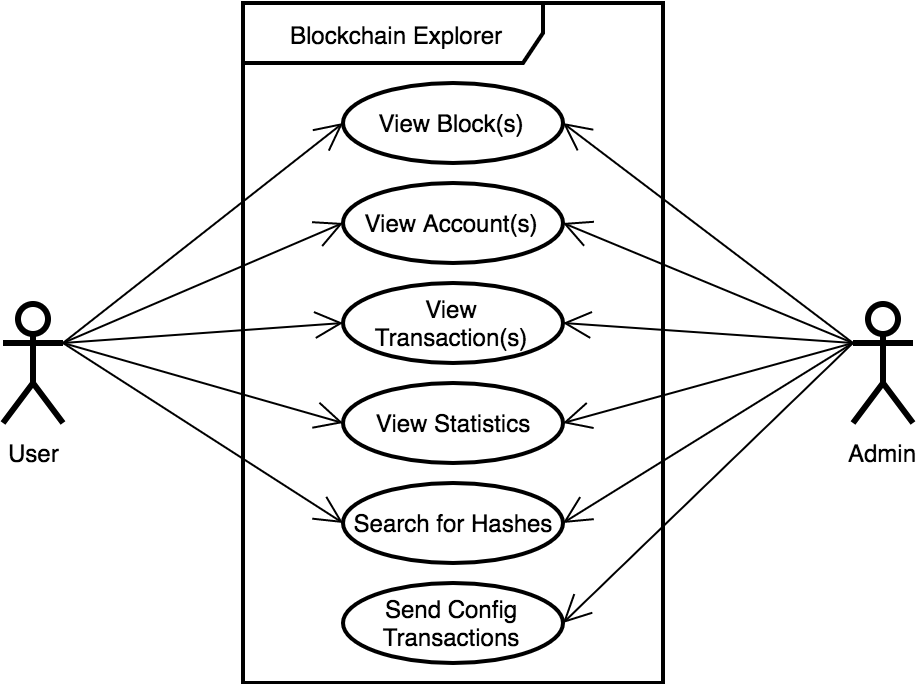
\includegraphics[width=\linewidth]{usecase1.png}
  \caption{Use Cases of the Block Explorer}
  \label{fig:usecase1}
\end{figure}

\section{Structure of the Service}
The program that users and admins use to view blockchain data is a website, which is made up of a front- and a backend. However, to run the blockchain explorer on its own, additional components beside the front- and backend programs are required. The website fetches blockchain data from an SQL database that runs independently from the blockchain. A separate database was chosen, because additional data like statistical information needs to be calculated and stored as well, which would bloat all miner?s built-in databases with information, if implemented in the miner. The fact that there are unified data structures and the possibility of having stored procedures in the database makes SQL a preferable database model, since the website always queries predefined statements. This also makes running the website possible without having a miner running in the backend. However this requires a program that copies data from a running Bazo mining node's database and stores it in the new  SQL database. As mentioned above, the backend accesses this database by making queries for relevant data and sending the results to the frontend to be displayed to the user.
\begin{figure}
  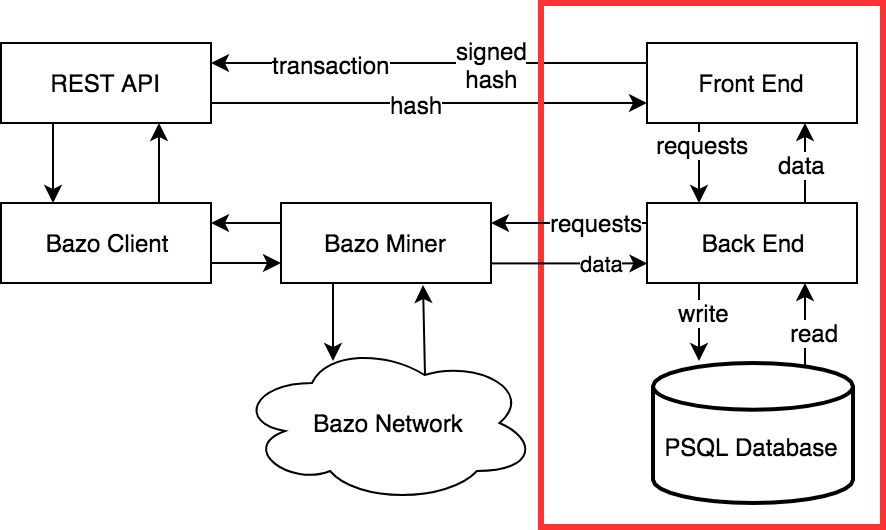
\includegraphics[width=\linewidth]{system.png}
  \caption{Structure of the Whole System}
  \label{fig:structure}
\end{figure}
\section{Structure of the Website}

\chapter{Implementation}
This chapter documents the implementation of the components listed in chapter \ref{chap:design}; Frontend, Backend and the SQL database. An additional section concerning hosting of the application on the internet is also included.
\section{Frontend}
XXX
\subsection{HTML Templates}
To interact with the Golang-Backend of the application, Gohtml templates have been used to define the markup of the application. One one hand, this makes way for a modular view component by letting programmers define reusable HTML modules such as headers, footers or table-templates. Using templates can minimize code duplication, which in turn makes maintenance on the code an overall less risky task. On the other hand, Golang templates allow for some limited logic in the Gohtml files, which is needed for handling variables that get passed from the backend component. For example, if the passed variable is an array of integers and the goal is to display all variables in a list, golang can create a new <li> tag for every value in the array. The HTML code that gets passed to the end user after making a request contains no Golang code, since the backend renders the Gohtml template files and passed variables to a useable HTML file that can be displayed by a web browser. Except for some Bootstrap functionality mentioned in \ref{sec:uiframeworks} and one case discussed in section \ref{sec:clientside}, all rendered pages of the application are static HTML files, because for every action a user may make on the website, a request has to be made to the backend. The website aims to always display the most recent data, so storing information that may not be up to date on the client's machine in order to save bandwidth, is outweighed by the possibility of having more recent data. 

\subsubsection{Reusable Modules}
lskjdflkj
\subsection{UI Frameworks} \label{sec:uiframeworks}
\subsection{Client-Side Logic} \label{sec:clientside}